%
% 
%
%%%%%%%%%%%%%%%%%%%%%%%%%%%%%%%%%%%%%%%%%%%%%%%%%%%%%%%%%%%%%%%%%%%%%%%%
\chapter{Fundamental Classes in CPPINTS}
%
%
%
In this chapter the fundamental classes in CPPINTS will be discussed in 
detail. These classes forms foundation for building the recurrence
relation(RR).

\section{Basis Set}
%
% 1  what's the form of basis sets?
% 2  why in basis set class we only store l,m,n information?
%
\label{bs}

In quantum chemistry, the basis set functions is the fundamental 
unit for practical calculations\cite{Davidson_Feller_CR_86_681_1986}. 
Primarily the basis set functions can be divided into radial part
and angular part. The radial part for the basis set function we discuss
in CPPINTS is formed by Gaussian functions, and the angular part could 
be further divided into two groups in terms of its function form.  
One group uses the spherical harmonics:
\begin{equation}
 \chi = Y_{m}^{L}(\theta,\phi)e^{-\alpha r^{2}}
\end{equation}
The other group uses the Cartesian function:
\begin{equation}\label{basis_set_cart_form}
 \chi = x^{l}y^{m}z^{n}e^{-\alpha r^{2}}
\end{equation}
In this program, we only focus on the Cartesian type
Gaussian basis set functions.

Generally the basis set function $\psi$ is a linear combination of 
Gaussian functions, and each such Gaussian function is also termed
as primitive function:
\begin{equation}\label{program_contract_basis_set}
	\psi = \sum_{\mu}d_{\mu}\chi_{\mu}
\end{equation}
$d$ is pre-optimized contraction coefficients.
$\chi_{\mu}$ is the primitive 
functions as defined in \ref{basis_set_cart_form}.
All of $\chi$ are on the same center as $\psi$, and they all share the 
same angular momentum with the basis set function.

For each basis set function, $x^{l}y^{m}z^{n}$ is its angular momentum part,
which is characterized by three number of l, m, and n. The $e^{-\alpha r^{2}}$
is its radial part, so l,m,n combined with exponential factor $\alpha$ and 
its coefficient of $d_{\mu}$; that give all of information to get $\psi$.

In the recurrence relation(RR), typically it starts with the bottom integral
\footnote{for VRR, bottom integral is in form of $(00|00)^{(m)}$ etc. For 
HRR, bottom integral is in form of $(0e|0f)$. See the chapter discussing RR 
for more information} and by raising up angular momentums it reaches the target
integrals. Therefore in the basis set class, we only use $l,m,n$ to represent 
the basis set.

In CPPINTS we also define the ``NULL'' basis set which means that 
this basis set is physical meaningless (l, m and n are all set to be -1). 
This type of basis set is used to complete an integral definition (see the 
\ref{integral} for more definition).

The basis set is defined in the file basis.cpp and basis.h.

%%%%%%%%%%%%%%%%%%%%%%%%%%%%%%%%%%%%%%%%%%%%%%%%%%%%%%%%%%%%%%%%%%%%%%%%
\section{Shell}
%
% 1  what's the shell? Why shell only have one data member of L?
% 2  what is the basis set order? How can we change it?
%
\label{shell}

In quantum chemistry, shell is an aggregation of same type of basis set
functions; whose total angular momentum is same(sum of l,m,n). For example, 
P shell contains 3 basis set functions, their l, m, n are characterized by:
\begin{align}\label{pshell_example}
	P_{x} &\Leftrightarrow (1,0,0) \nonumber \\
	P_{y} &\Leftrightarrow (0,1,0) \nonumber \\
	P_{z} &\Leftrightarrow (0,0,1)
\end{align}
By following the same principle, it's able the form D shell ($L = l+m+n = 2$), 
F shell ($L = l+m+n = 3$) etc.

As what we have demonstrated in the basis set functions section, to fulfill
recurrence relation it only requires the angular momentum information. 
Therefore, in the shell class it's only the total angular momentum L
is defined.

Here it needs to emphasize that how to arrange the basis set
functions in a given shell, this is called ``basis set order''.
For example, for the P shell, it's able to have:
\begin{equation}
 P_{x} \Rightarrow P_{y} \Rightarrow P_{z}
\end{equation} 
or the other order of 
\begin{equation}
 P_{z} \Rightarrow P_{y} \Rightarrow P_{x}
\end{equation} 

Since different basis sets in a shell are in a same level, therefore
there's not a basis set order prior to the others. It's able to 
pick up any basis set order theoretically. In this program, we 
pick up the ``libint'' order (which is used by libint program
\footnote{\url{http://sourceforge.net/projects/libint/}}). 
In basisutil.h, the arrangement of basis set order is given for 
L up to 20. On the other hand, it's able to use the other 
type of basis set orders. Therefore we separate the basis set 
order information all into the basisutil.h and basisutil.cpp.

In terms of a given basis set order, each basis set occupies an
unique position in the 
basis set order array, which refers as ``local index'' of the 
basis set in the given shell. For example, in the above P shell
case \ref{pshell_example} $Px$ is 0, $Py$ is 1, $Pz$ is 2. For 
each basis set it's able to set up some ``ONE-TO-ONE'' mapping 
relation between basis set and it's position in the basis set 
order list. Such fundamental relation is used for building the 
mapping relation between shell quartet and integral (see 
section \ref{mapping_integral_sq} for more details).

If the user wants to employ other type of basis set order other 
than the libint order, here is the procedure the user should
follow:
\begin{itemize}
 \item generate all of explicit basis set order array and 
	 replace the old content of ``LIBINT\_BASIS\_SET\_ORDER''
	 with the new array (this is in basisutil.h). This step
	 will enable you to get correct basis set by given 
	 a basis set index;
 \item Secondly the function of ``getLocalBasisSetIndex'' in
	 basisutil.cpp should be updated for the new basis 
	 set order. This step will give the correct local index
	 by an arbitrary input l, m, n value of basis set.
\end{itemize}
Now the mapping between index and angular momentum should 
set up. You should get correct integral results without 
referring to the other places.

Similar with basis set, we also define ``NULL'' shell whose 
L is set to be -1. This type of shell is used to complete 
shell quartet definition.

The shell is defined in shell.h and shell.cpp.

%%%%%%%%%%%%%%%%%%%%%%%%%%%%%%%%%%%%%%%%%%%%%%%%%%%%%%%%%%%%%%%%%%%%%%%%
\subsection{Composite Shells}
%
% 1  what is the composite shell?
% 2  how we handle the composite shell? 
\label{composite_shell}
%
%
The composite shell is that for each shell it may contain several
type of sub-shells. For example, SP shell has one S shell and one 
P shell, and SPD shell has S shell, P shell and a D shell. All of 
these sub-shells share the same exponential factors for it's radial part,
and each of them has its own contraction coefficients of $d$ in equation
\ref{program_contract_basis_set}. The most famous basis set library using 
composite shell is Pople basis sets (6-31G etc.)

In our program, the shell class is defined for ``pure'' shell(shell that
only corresponds to one $L$ value) and the composite shell situation is 
handled elsewhere. You can refer to the section \ref{composite_shell_quartet} 
etc. for more details that how CPPINTS handle the composite shell situation.

%%%%%%%%%%%%%%%%%%%%%%%%%%%%%%%%%%%%%%%%%%%%%%%%%%%%%%%%%%%%%%%%%%%%%%%%
\section{Integral Type}
%
% how to represent the integral operator?
%
\label{inttype}

In CPPINTS, we have a series of pre-defined integer to represent 
the ``OPERATORS'' used in quantum chemistry integrals. For example,
the two body overlap integral(TOV), nuclear-electron attraction integral(NAI)
etc. These integers are defined in the inttype.h and inttype.cpp(it's 
name appears as macro defined in general.h). The pre-defined integral 
is a data member for both integral and shell quartet class.

For the given integral type, there are some integral properties that 
is solely determined by the integral operator itself. For example,
NAI is two body integral, and it requires $(0|0)^{(m)}$ for RR etc.
You can find the details from inttype.cpp that what kind of properties 
can be determined only from operator itself.

%%%%%%%%%%%%%%%%%%%%%%%%%%%%%%%%%%%%%%%%%%%%%%%%%%%%%%%%%%%%%%%%%%%%%%%%
\section{Integral and Shell Quartets}
%
% 
%
%%%%%%%%%%%%%%%%%%%%%%%%%%%%%%%%%%%%%%%%%%%%%%%%%%%
\subsection{Integral}
\label{integral}
%
% 1  what is integral?
% 2  how to represent it?
%
For a given operator representing quantum quantity (for example,
the kinetic operator, electron repulsion operator etc.) it's able 
to form the integrals based on the basis set functions:
\begin{equation}
 I = \langle \psi_{l_{1}m_{1}n_{1}}(r)\psi_{l_{2}m_{2}n_{2}}(r)| 
 \hat{f}(r,r^{'})| \psi_{l_{3}m_{3}n_{3}}(r^{'})
 \psi_{l_{4}m_{4}n_{4}}(r^{'})\rangle
\end{equation}
therefore to define an integral, basically the following 
information is needed:
\begin{itemize}
 \item operator;
 \item basis set information for all given integral positions
\end{itemize}
Because recurrence relation also uses the integrals $(ab|cd)^{(m)}$,
an additional $m$ value is defined in both integral and shell
quartet class.

Primarily the integrals could be divided into different categories according 
to the number of its basis set function components. In quantum chemistry, 
the possible number of basis set functions in the integral is ranging 
from 1 to 4. Therefore, integral is ranging from one body integral to 
four body integrals. 

The four possible basis set positions are called as: ``BRA1'', ``BRA2'',
``KET1'' and ``KET2''. For one body integral, it's only the bra1
position having basis sets(other positions have null basis set); 
for the two body integral, it's only bra1 and bra2 positions having 
basis sets; for the three body integral, 
it's only bra1, bra2, and ket1 positions having basis sets. 
Such position definition is used across the whole program, and the 
similar definition holds for shell quartet, too.

The integral class always has four position for the basis set (see 
integral.h). For the one to three body integrals, we use NULL
basis set to complete the integral definition.

The integral is defined in integral.cpp and integral.h.
%%%%%%%%%%%%%%%%%%%%%%%%%%%%%%%%%%%%%%%%%%%%%%%%%%%
\subsection{Shell Quartet}
%
% how to define shell quartet?
% what is the relation between shell quartet and integral?
%
\label{shell_quartet}
Similar to the relation between basis set and shell, the aggregation 
of certain type of integrals will lead to the ``shell quartet''.

For example, for the electron repulsion operator it's able to define 
the shell quartet over four shells:
\begin{equation}
 SQ_{P,P,P,P} = \langle P_{bra1}P_{bra2}|
 \frac{1}{r_{12}}|P_{ket1}P_{ket2} \rangle
\end{equation}
This shell quartet includes all of integrals in terms of basis sets
for the given four P shells. Because each P shell have 3 basis set
functions, the shell quartet contains $3^{4} = 81$ ERI integrals.

Similar to the integral class which is defined based on the basis set
class; the shell quartet is constructed based on the shell class. Therefore
for defining a fundamental shell quartet, it needs shell information
on all of four BRA1, BRA2, KET1 and KET2 positions (null shell is used
to complement the shell quartet definition) as well as the operation
information.

The definition of shell quartet could be referred to shellquartet.h
and shellquartet.cpp.

%%%%%%%%%%%%%%%%%%%%%%%%%%%%%%%%%%%%%%%%%%%%%%%%%%%
\subsection{Mapping between Integral and Shell Quartet}
\label{mapping_integral_sq}

For CPPINTS, shell quartet is the basic unit for deriving the 
recurrence relation. The integrals are considered to be attached to 
its corresponding shell quartet.

Based on the ``ONE-TO-ONE'' mapping relation between basis set 
and shell, it's able to construct the ``ONE-TO-ONE'' mapping relation
between integral and its shell quartet. For each integral, it 
has a unique position according to the given basis set order.
For example, integrals in the shell quartet $(SPSP|SPSP)$ may 
correspond to an order like:
\begin{align}
 (SS|SS)         &\rightarrow  0 \nonumber \\
 (P_{x}S|SS)     &\rightarrow  1 \nonumber \\
 (P_{y}S|SS)     &\rightarrow  2 \nonumber \\
 (P_{z}S|SS)     &\rightarrow  3 \nonumber \\
 (SP_{x}|SS)     &\rightarrow  4 \nonumber \\
 (P_{x}P_{x}|SS) &\rightarrow  5 \nonumber \\
 (P_{y}P_{x}|SS) &\rightarrow  6 \nonumber \\
 (P_{z}P_{x}|SS) &\rightarrow  7 \nonumber \\
                 &\cdots
\end{align}
By giving the shell quartet and this unique position, it's able 
to reconstruct the integral; on the other hand, from the given 
integral it's able to derive its unique position\footnote{please
refer to integral.cpp for more details that how we do it}.

%%%%%%%%%%%%%%%%%%%%%%%%%%%%%%%%%%%%%%%%%%%%%%%%%%%
\subsection{Representation of Integral in Recurrence Relation}
%
% why we use position ID to reprernt integral in shell quartet?
%
\label{representation_integral_sq}

The ``ONE-TO-ONE'' mapping relation could be used to improve the memory 
usage for CPPINTS. Suggest we have a $(II|II)$ ERI shell 
quartet for deriving its vertical recurrence relation, to record
all of the information for each integrals requires the following 
items:
\begin{itemize}
 \item LHS integral;
 \item RHS integral and its coefficients.
\end{itemize}

For each integral, to characterize it it requires $3\times 4 = 12$
integers to record angular momentum information, plus two integers
for operator and m value. Therefore each integral needs 14 integer
\footnote{we have not considered the division yet, which is related to
composite shell quartet case}.

For the OS VRR framework, the recursive relation has 8 items on the 
RHS so there are totally 9 integrals, which needs 126 integers. 
Because the $(II|II)$ has $28^4$ integrals, it needs 77446656 integers.
Suggest each integer takes 4 byte memory, the total memory for 
storing integer of this shell quartet would be 296mb! So far we did not
count in the coefficients.

However, if we use the ``position ID'' to represent the integrals 
inside the shell quartet, then each integral only need one integer 
thus it's only 5.3mb memory needed. Therefore, to use the position 
ID to represent integrals inside shell quartet is a good way for 
memory saving with only marginal CPU cost added. This is the way
we handle integrals in the recurrence relation(RR) process.

%%%%%%%%%%%%%%%%%%%%%%%%%%%%%%%%%%%%%%%%%%%%%%%%%%%
\subsection{Composite Shell Quartet}
%
%
\label{composite_shell_quartet}

In a given shell quartet, if one of its shell is in composite type; 
then this shell quartet is composite shell quartet. It contains
several shell quartets in terms of pure shell. For example,
shell quartet $(DD|DSP)$ has two pure shell quartets; namely 
$(DD|DS)$ and $(DD|DP)$.

How to process composite shell quartet in the recurrence relation?
It's depending on whether it's HRR or it's in VRR.

For VRR, Let's take ERI as example. Because the recurrence relation 
is generally expressed as: 
\begin{align}
I(L,m) &= a_{0}I_{0}(L-1,m) + a_{1}I_{1}(L-1,m+1) \nonumber \\ 
&+ a_{2}I_{2}(L-2,m) - a_{3}I_{3}(L-2,m+1) \nonumber \\
&+ a_{4}I_{4}(L-2,m) - a_{5}I_{5}(L-2,m+1) \nonumber \\
&+ a_{6}I_{6}(L-2,m+1) + a_{7}I_{7}(L-2,m+1)
\end{align}
The above integral expression is on primitive Gaussian function, and 
$a_{i}$ is RR coefficient which is independent with the integral.
Because VRR is linear with the contraction coefficients $d$,
the expression above holds for both contracted and un-contracted primitive
Gaussian functions. Therefore, the recurrence relation for VRR is 
independent of the contraction information. We can simply get the 
integral with contraction coefficients by multiply it to the final
results:
\begin{equation}\label{composte_sq_contraction_coefs}
 I_{contracted}(L,m) = d_{bra1}d_{bra2}d_{ket1}d_{ket2}I(L,m)
\end{equation}
This is what we do for dealing with the composite shell quartets in VRR.
Because in composite shell the sub-shells share the same exponential
factor, the raw integral $I(L,m)$ in \ref{composte_sq_contraction_coefs} 
is same between different pure shell quartets; the final integral results
with contraction coefficients could be simply retrieved by performing 
\ref{composte_sq_contraction_coefs}. This is called ``contraction'' step
in VRR. The pseudocode is given like this:
\begin{verbatim}
loop over ket side primitive Gaussian pairs:
  loop over bra side primitive Gaussian pairs:
    compute bottom integrals;
    do VRR to derive result integrals;
    perform contraction step; 
  end loop
end loop
\end{verbatim}
For pure shell quartet like $(DD|DD)$, there's no need to perform 
contraction step because it can simply add contraction information
to the bottom integrals $(00|00)^{(m)}$ so that VRR is performed 
for contracted integrals. After VRR is ending, the result integrals
get updated by the result in the primitive integral loops.

However, for HRR the story is different. Because HRR is usually applied on
contracted integral results (it sums over all of integrals on 
primitive Gaussian functions), the equation \ref{composite_sq_hrr}
shows that how we can step from
un-contracted integrals to contracted ones in HRR:
\begin{align}\label{composite_sq_hrr}
 [a(b+\iota_{i})|cd]_{k} &= [(a+\iota_{i})b|cd]_{k} + 
(A_{i} - B_{i})[ab|cd]_{k} \rightarrow \nonumber \\
\sum_{k}C_{k}[a(b+\iota_{i})|cd]_{k} &= \sum_{k}C_{k}[(a+\iota_{i})b|cd]_{k} + 
(A_{i} - B_{i})\sum_{k}C_{k}[ab|cd]_{k} \rightarrow \nonumber \\
(a(b+\iota_{i})|cd) &= ((a+\iota_{i})b|cd) + 
(A_{i} - B_{i})(ab|cd)
\end{align}
Here $[ab|cd]$ is used to represent the integrals on un-contracted Gaussian 
functions, and $(ab|cd)$ for the contracted integrals; $C_{k}$ is the 
combination for all of contraction coefficients of $d$.

It's clear from \ref{composite_sq_hrr} that as long as LHS and RHS share the 
same contraction coefficients, HRR can be applied from $(0e|0f)$ until
the final target integral $(ab|cd)$ is derived. Hence for the composite 
shell quartets, each pure shell quartet has its own HRR process and they
are independent with each other.

For this reason, we have a data member named as ``division'' on both
integral and shell quartet classes. It's an ID for each pure shell quartet
in the composite shell quartet. For example; $(DSP|DSP)$ has four shell quartets;
$(DS|DS)$, $(DS|DP)$, $(DP|DS)$ and $(DP|DP)$ and each pure shell quartet has it's 
own ID number (characterized by division). They will have their own
HRR process.

%%%%%%%%%%%%%%%%%%%%%%%%%%%%%%%%%%%%%%%%%%%%%%%%%%%
\subsection{Sorting Shell Quartets}
%
%
\label{sort_shell_quartet}

After RR(VRR or HRR) path is constructed in detail, a sorting 
function is needed to be applied to the whole LHS shell quartets
so that to make sure all of RHS shell quartets are well defined
in the previous content. Therefore, we need sorting function for 
building the correct RR.

The inconvertibility character for VRR establishes in section 
\ref{optimal_path} in fact enables us to set up sorting facility
on the shell quartet in the RR direction. In other words, in 
accumulating all of RR terms along the VRR path; we are able 
to sort the shell quartets either from bottom integrals to
the results(this is always from RHS to LHS in terms of RR),
or from the results to the bottom integrals in reverse.

This is what the operator $<$ function in shell quartet class
does. By following the VRR formula\footnote{right now the function
just follows the VRR in OS framework}, it's able to distinguish
the shell quartet on either RHS or LHS. More details can be 
found in the comments of this function.

HRR does not hold the inconvertibility character as shown in 
section \ref{optimal_path}. However, it's still applicable 
to set up some algorithm to sort the shell quartets in the 
HRR process. The sorting function for HRR is presented in
hrrCompare function in shellquartet.cpp. Therefore, it's 
able to sort the HRR shell quartets so that we print out 
the HRR formula in correct order.


%%%%%%%%%%%%%%%%%%%%%%%%%%%%%%%%%%%%%%%%%%%%%%%%%%%%%%%%%%%%%%%%%%%%%%%%
\chapter{Core Concepts of CPPINTS}


%%%%%%%%%%%%%%%%%%%%%%%%%%%%%%%%%%%%%%%%%%%%%%%%%%%%%%%%%%%%%%%%%%%%%%%%
\section{Introduction to Analytical Integral Algorithms}
\label{concepts_introduction}

The integral we discussed here is analytical integrals,
which is generally expressed as:
\begin{equation}\label{int_paper:1}
  I_{ijkl} = \int \chi_{i}(\bm{r})\chi_{j}(\bm{r})f(\bm{r},\bm{r^{'}})
\chi_{k}(\bm{r^{'}})\chi_{l}(\bm{r^{'}}) d\bm{r} d\bm{r^{'}}
\end{equation}
and the integrand is analytically integrated. Kinetic integrals(KI),
nuclear attraction integrals(NAI), electron repulsion integrals(ERI) etc. all 
belong to this group. 

Since Boys\cite{SFBoys1950} suggested to use Cartesian Gaussian type function to form 
basis functions,
\begin{equation}\label{int_paper:2}
 \chi = x^{i}y^{j}z^{k}e^{-\alpha r^{2}}
\end{equation}
a major breakthrough technology for computing ERI was introduced by Pople and Hehre(PH)\cite{PH}. 
This method provides exceptional efficient algorithm for computing high contracted 
low angular momentum integrals. However, this method is limited to S and P basis functions, 
and it's difficult to be extended to high angular momentum integrals. McMurchie and 
Davidson(MD)\cite{MD}
proposed a general formalism for computing variety kind of analytical integrals in terms of 
Hermitian polynomials, and their method is applied to integrals with high angular momentum. 
Dupuis, Rys and King(DRK)\cite{DRK1976JCOMP,DRK1976JCP,DRK1983JCOMP} developed another formalism 
for ERI based on exact numerical 
quadrature using root and weights generated from Rys polynomials. Although MD and DRK
methods provide general way to derive the analytical integrals, they are indirect methods where
auxiliary polynomials need to be involved. 

In 1980s, Obara and Saika(OS)\cite{OS1986,OS1988} derived a set of
recursive formulas for analytical integrals based on recursive expression of 
three body overlap integral. In the OS method it's able to directly generate the integrals. The 
recurrence relation(RR) for ERI in OS scheme is given as:
\begin{equation}
 \begin{split}
((a+\iota_{i})b|cd)^{(m)} &= (P_{i} - A_{i})(ab|cd)^{(m)} +
\left(W_{i} -P_{i}\right)(ab|cd)^{(m+1)} \\
&+\frac{N_{i}(A)}{2\epsilon}\left(((a-\iota_{i})b|cd)^{(m)}-\frac{\rho}{
\epsilon }((a-\iota_{i})b|cd)^{(m+1)}\right)  \\
&+\frac{N_{i}(B)}{2\epsilon}\left((a(b-\iota_{i})|cd)^{(m)}-\frac{\rho}{
\epsilon }(a(b-\iota_{i})|cd)^{(m+1)}\right)  \\
&+\left(\frac{N_{i}(C)}{2}\right)\frac{1}{\epsilon+\eta}
(ab|(c-\iota_{i})d)^{(m+1)} \\
&+\left(\frac{N_{i}(D)}{2}\right)\frac{1}{\epsilon+\eta}
(ab|c(d-\iota_{i}))^{(m+1)}
\end{split}
\label{int_paper:3}
\end{equation}
where the $(ab|cd)^{(m)}$ is:
\begin{equation}
\label{int_paper:4}
 (ab|cd)^{(m)} = \frac{2}{\sqrt{\pi}}\int^{\infty}_{0} du \left( \frac{u^{2}}
{\rho+u^{2}}\right)^{m}(ab|u|cd) 
\end{equation}
$(ab|cd)^{(0)}$ is the result ERI of $(ab|cd)$. In the OS scheme to compute an arbitrary ERI 
of $(ab|cd)$, the bottom integrals of $(00|00)^{(0)}$, $(00|00)^{(1)}$ etc. are needed 
to be evaluated first; through the recursive expansion \ref{int_paper:3} it's able to raise
up the angular momentum recursively until the target integral $(ab|cd)$ is derived. Lindh, 
Ryu and Liu\cite{lindh1991reduced}(LRL) proposed a similar RR based on Rys 
polynomials. Because the integrals are calculated in ``vertical'' way, 
such methods are named as ``vertical recurrence relation''(VRR).

In contrast to the VRR, Head-Gordon and Pople(HGP)\cite{HGP} found another general formula which 
performs ``horizontal recurrence relation''(HRR) on analytical integrals. In HRR the ERI
is evaluated as:
\begin{equation}
\label{int_paper:5}
 (a(b+\iota_{i})|cd) = ((a+\iota_{i})b|cd) + 
(A_{i} - B_{i})(ab|cd)
\end{equation}
Consequently the ERI $(ab|cd)$ can be recursively derived from a set of auxiliary integrals
in form of $(e0|f0)$. Because the HRR only involves the basis function centers,
it can be applied to contracted integrals thus to save computation cost 
inside the contraction loop. Hamilton and Schaefer\cite{new_hrr_Schaefer}(HS) derived a 
similar HRR by using translational invariance condition, it shifts the integral in form of 
$(a+b+c+d0|00)$ to $(a+b0|c+d0)$. 

For practical integral evaluation, HRR needs to combine with other
methods to finish the whole integral derivation. HGP\cite{HGP} scheme combines the HRR with OS scheme,
Gill etc. \cite{gill1989efficient, gill1990efficient}suggested to join HRR and MD methods together. 
Other type of combinations are also proposed\cite{lindh1991reduced,new_hrr_Schaefer}.

%%%%%%%%%%%%%%%%%%%%%%%%%%%%%%%%%%%%%%%%%%%%%%%%%%%%%%%%%%%%%%%%%%%%%%%%
\section{Primary Achievement of CPPINTS}
%
%
%
Although VRR provides clear formalism for recursively generating integrals, it's still 
uncertain that how to generate the integrals with least amount of work. This problem is 
referred as ``tree-search problem''\cite{HGP}. Generally in the VRR, the recurrence derivation on 
ERI forms a ``directed graph'' data structure\footnote{see 
\url{http://en.wikipedia.org/wiki/Directed_graph} for more details} as shown in figure \ref{fig:1}. 
The tree-search problem is to find the optimal directed graph(or commonly referred as path) with 
minimum of work, for example; with minimum FLOPS or with minimum number of intermediate variables. 

 \begin{figure}[htb]
 \centering
 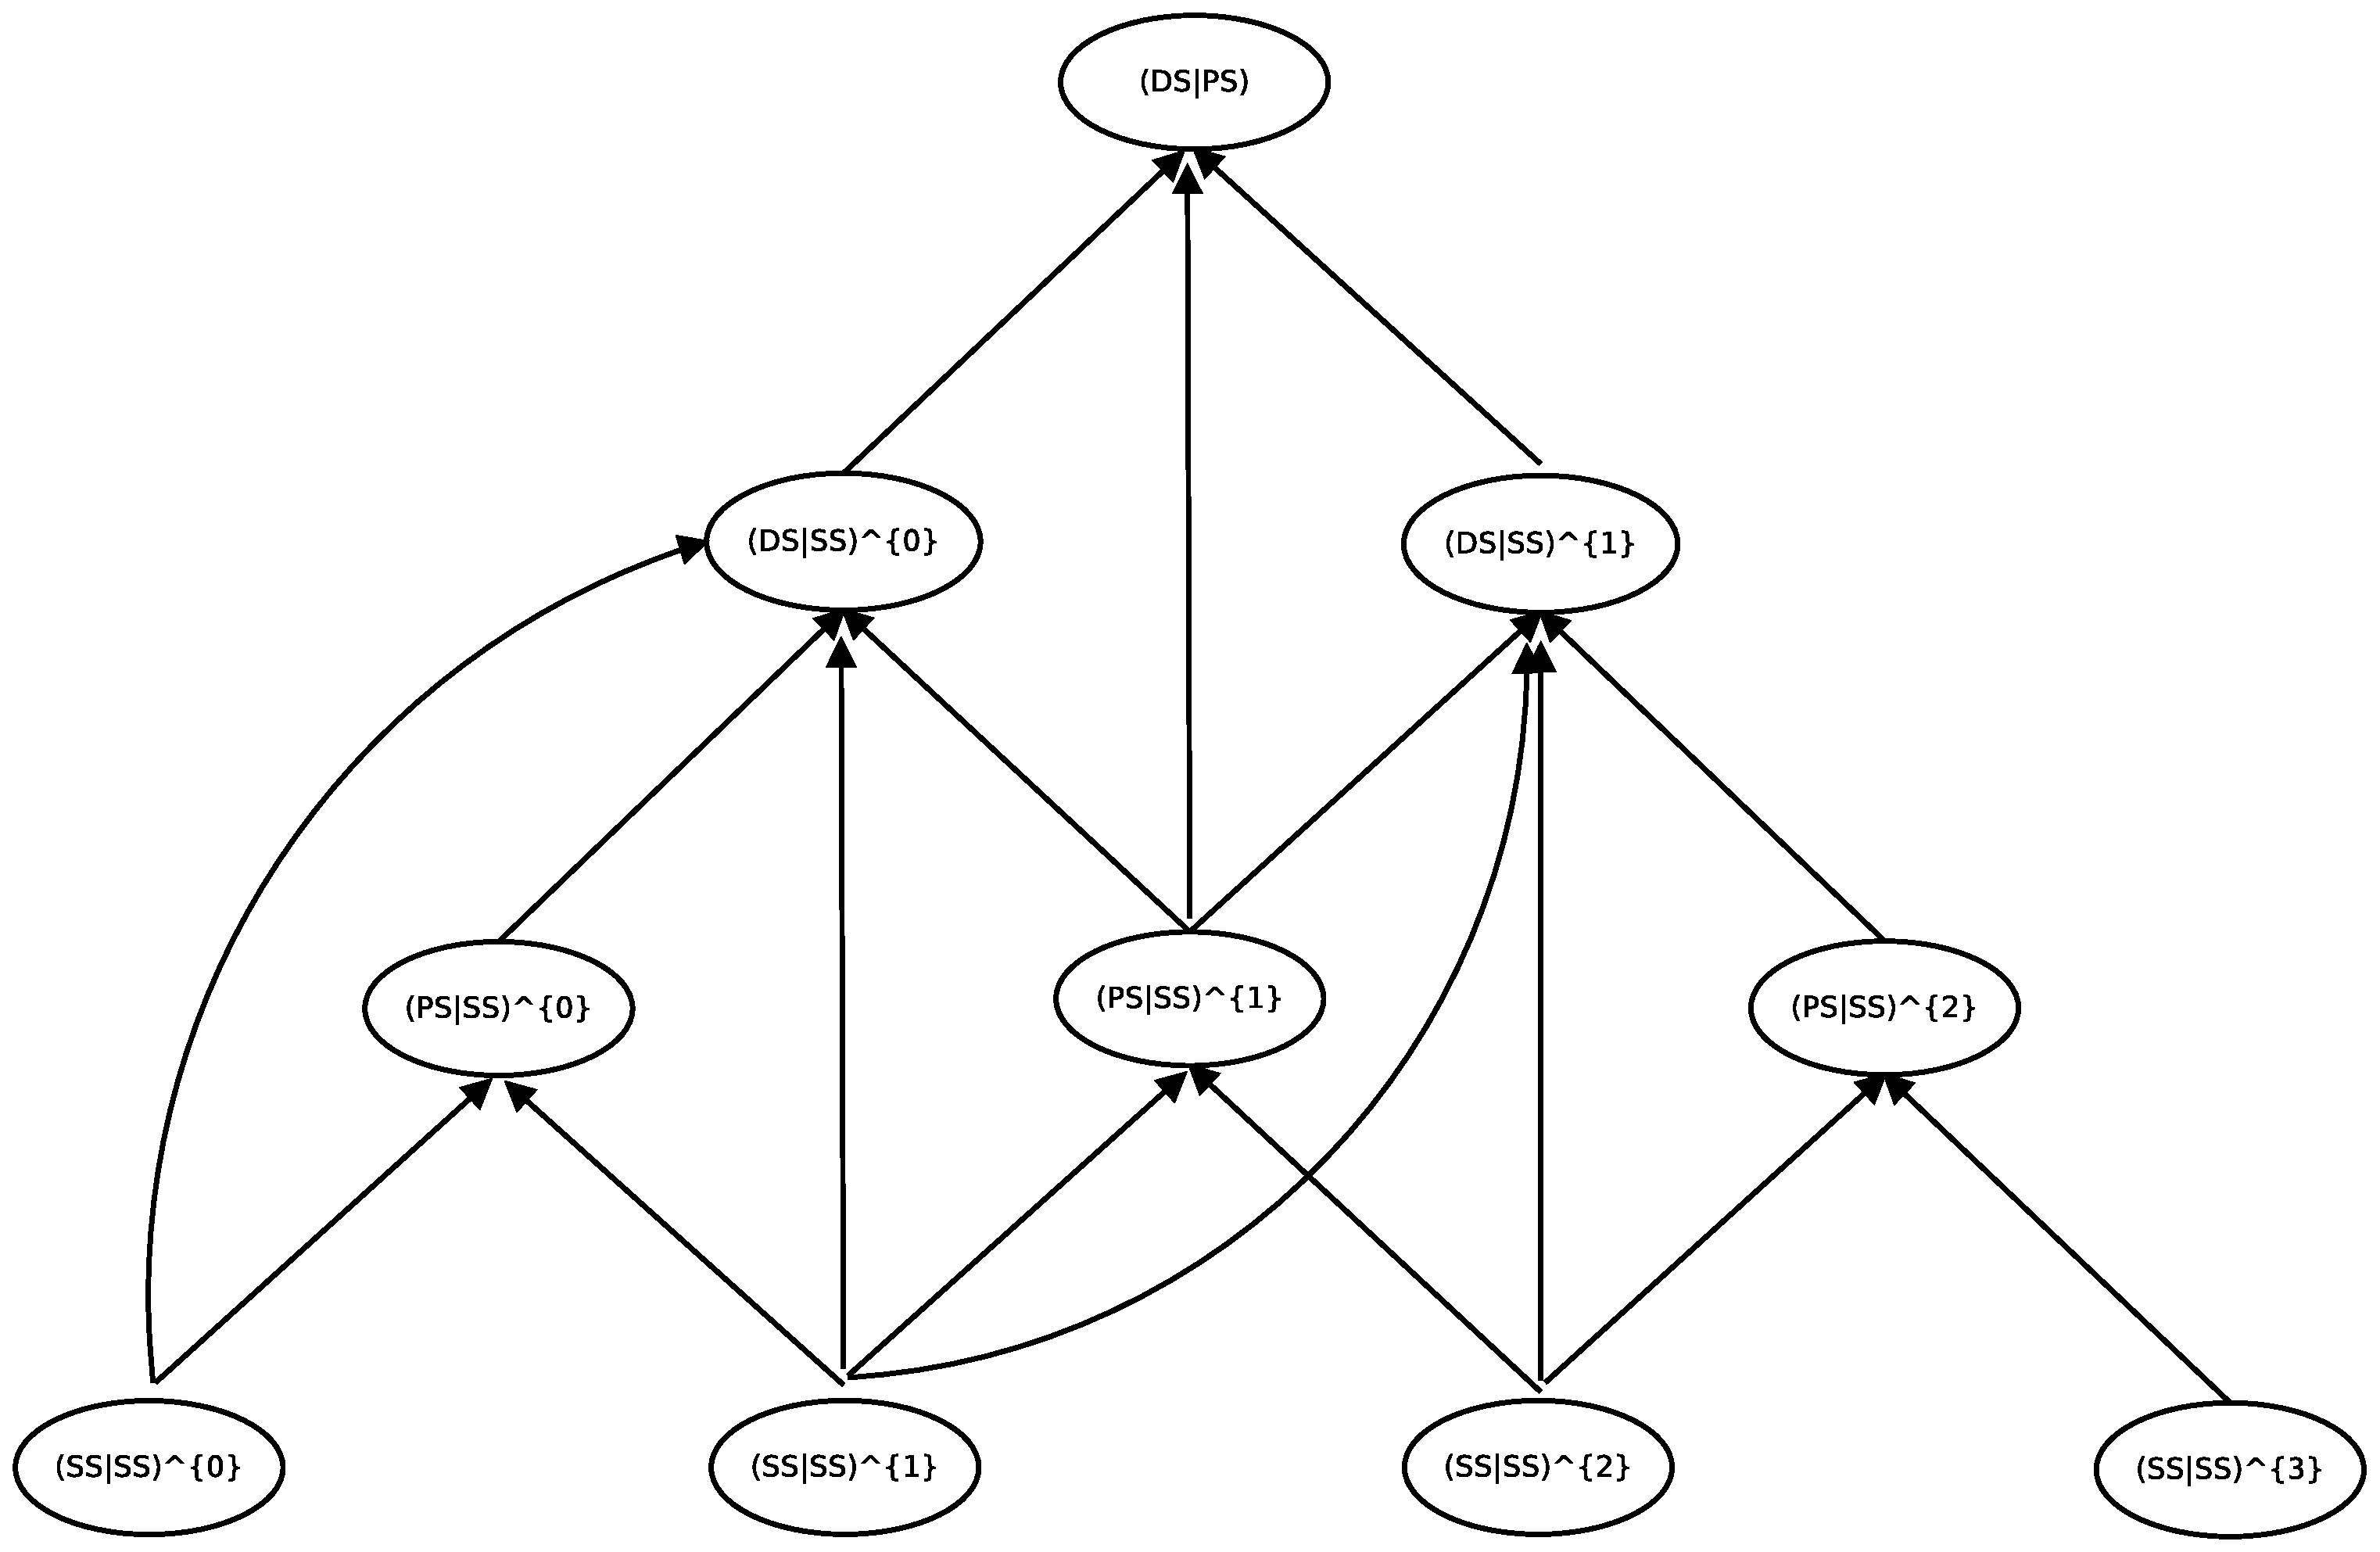
\includegraphics[scale=0.25]{./graph.eps}
 % general_rr.eps: 0x0 pixel, 300dpi, 0.00x0.00 cm, bb=0 0 763 487
 \caption{directed graph for integral of $(DS|PS)$ based on OS scheme}
 \label{fig:1}
\end{figure}

In CPPINTS, a general searching algorithm is used on solving the tree-search problem for 
VRR. Instead of exploring details for optimal path, by
investigating the nature of VRR formula we can wrap up correlated integrals into packages
and it turns out that the packages are independent with each other on the VRR path. Based on
the concept of package, the directed graph for VRR is converted into tree data structure and the optimal
path for VRR is corresponding to the shortest path in the given tree data structure, where the
a similar Dijkstra's algorithm\footnote{please see 
\url{http://en.wikipedia.org/wiki/Dijkstra\%27s_algorithm} for more information} is applied.
This part will be discussed in section \ref{optimal_path}.

For computing the target integrals, both VRR and HRR need many intermediate integrals on
the recurrence relation(RR) path. The interesting question is, is every intermediate integral 
necessary in the recurrence generation? The question becomes more interesting in terms of 
the redundancy of Cartesian type of Gaussian functions in comparison with the spherical form of 
Gaussian functions. In the section \ref{redundancy_rr} a general recursive procedure is 
employed to explore the redundancy of RR.


%%%%%%%%%%%%%%%%%%%%%%%%%%%%%%%%%%%%%%%%%%%%%%%%%%%%%%%
% optimal VRR path
%%%%%%%%%%%%%%%%%%%%%%%%%%%%%%%%%%%%%%%%%%%%%%%%%%%%%%%
\section{Finding Optimal Path for Recurrence Relation}
\label{optimal_path}

The optimal path for RR can be defined in variety of way. In this paper,
the optimal path is the implementation of RR with minimum intermediate integral
number. Our discussion below is based on HGP scheme above. However,the idea 
and implementation below is easy to transfer to other RR schemes.

In the practical implementation of RR, the integral calculation is usually performed 
in terms of shells rather than basis functions, so that to reduce the repeat use of 
intermediate integral. Considering the equation \ref{int_paper:3}, 
all of shell positions in the shell quartet $(FD|PS)$ are expandable except the ``ket2'' position 
where the shell is ``S'' type of 
function. Therefore for each LHS ERI appearing in the VRR, how to find it's proper expandable
position so that to minimize the total number of intermediate integrals is the key to 
find optimal path for VRR.

Let's take ERI as an example. The equation \ref{int_paper:3} can be generalized into a 8-term 
expansion:
\begin{align}\label{int_paper:7}
I(L,m) &= a_{0}I_{0}(L-1,m) + a_{1}I_{1}(L-1,m+1) \nonumber \\ 
&+ a_{2}I_{2}(L-2,m) - a_{3}I_{3}(L-2,m+1) \nonumber \\
&+ a_{4}I_{4}(L-2,m) - a_{5}I_{5}(L-2,m+1) \nonumber \\
&+ a_{6}I_{6}(L-2,m+1) + a_{7}I_{7}(L-2,m+1)
\end{align}
$L$ is the sum of angular momentum
\begin{equation}\label{int_paper:8}
 L = L_{a} + L_{b} + L_{c} + L_{d}
\end{equation}
for ERI $(ab|cd)$, and $m$ is the parameter for auxiliary integral $(ab|cd)^{(m)}$ in 
expression \ref{int_paper:4}.
From equation \ref{int_paper:7}, it's clear that the $L$ is constantly decreasing and $m$ is
increasing in same manner from LHS to RHS. Therefore the properties of $L$ and $m$ 
for ERI characterize an ``arrow'' in the derivation of VRR, in this sense the VRR
for ERI is ``inconvertible'' between LHS and RHS. As see in the following discussion,
such inconvertibility grantees the existence of conversion for transforming the graph
data structure into the tree data structure for ERI\footnote{In tree data structure,
every children node can only have one parent node. Such character establishes the direction
of the tree. Please see \url{http://en.wikipedia.org/wiki/Tree_\%28data_structure\%29} for 
more information}, and it also establishes an order 
of sequence between two arbitrary ERI so that RHS ERI is always generated prior to
the LHS ERI in the resulting VRR path.

Based on the feature of inconvertibility, it's able to set up some general coding structure
to perform the optimal path search for ERI in VRR (unsolved shell quartets are these who
appear in VRR path but their expanding position are not yet determined):
\begin{verbatim}
set up unsolved shell quartet archive;
initilize the unsolved shell quartet archive with 
input LHS shell quartets;
loop over m (from m=0 to maximum):
  loop over L (from maximum to 0):
    while(true):
      perform optimal expanding postion search for 
      all (L,m) LHS shell quartets in the unsolved 
      shell quartet archive;
      if there are no (L,m) LHS shell quartets break 
      out the loop;
    end while
  end loop with L
end loop with m
\end{verbatim}
The search is carried out from the LHS to RHS until all of LHS shell quartets 
are solved. The procedure here establishes a general Dijkstra algorithm scheme 
for searching expanding positions for VRR. By wrapping up all of unsolved 
$(L,m)$ shell quartets together, it's able to search their their optimal expansions
and the following search iteration will be performed based on the output of
previous iterations. 

How to evaluate the efficiency of the algorithm comparing with Breadth-first search
or Depth-first search across all of possible VRR paths? In general the Dijkstra algorithm
can not guarantee a global minimum because the global minimum may not be reached by
by assembling minimums on the partial path. However, because L is constantly decreasing
from LHS to RHS; the integral numbers are constantly decreasing from current search
iteration to the following ones. Therefore it could expect that the above procedure
may give the close VRR path comparing with the global optimum.

In terms of an arbitrary given unsolved $(L,m)$ shell quartets, all of shell quartets
appearing in VRR can be divided into three groups:
\begin{itemize}
 \item unsolved main list;
 \item correlated list;
 \item irrelevant list 
\end{itemize}
Unsolved main list contains the unsolved shell quartets with given properties of $(L,m)$.
Their expanding position are going to be determined in the current iteration of search. 
Correlated list is composed by the unsolved shell quartets who possibly share the RHS 
terms with the unsolved main list. The irrelevant list is composed by all of other 
unsolved shell quartets and their expansion positions are independent with the 
unsolved main list. By combining the unsolved main list and correlated list together 
to form a package, all of correlated LHS shell quartets are self-contained therefore 
it's able to carry out a full search on all possible expansion combinations for every 
LHS shell quartets inside the package. The search result gives the final expanding
positions to the unsolved main list.

Let's take ERI as illustration. The VRR in equation \ref{int_paper:7} demonstrates that 
for ERI $I(L,m)$, only ERI of $I(L-1,m)$, $I(L,m+1)$ and $I(L-1,m+1)$ can share RHS with it.
These ERI are in unsolved state and their undetermined expansion will affect the determination 
of expanding position for $I(L,m)$. On the other hand, although ERI with $L+1$ or $m-1$ are 
also possibly sharing RHS with $I(L,m)$, their expanding position have been solved in previous 
iteration; therefore these shell quartets apply deterministic effects on the search of expanding 
position searching for ERI $I(L,m)$. As a result of inconvertibility of VRR, the number of shell
quartets which constitutes the correlated package decreases significantly.

In summary, for searching the expanding position of shell quartets with property of $(L,m)$, 
it's able to form an independent package with unsolved shell quartets characterized by property 
$(L-1,m)$, $(L,m+1)$ and $(L-1,m+1)$. A complete survey to find minimum RHS integrals for $(L,m)$
shell quartets is performed in terms of all of possible expansion combinations for all of shell 
quartets inside the package. The implementation for the above algorithm is depicted as below:
\begin{verbatim}
set up archive for solved shell quartets;
set up archive for unsolved shell quartets;
initilize the unsolved archive with input shell quartets;

loop over m (from m=0 to maximum):
  loop over L (from maximum to 0):
    while(true)
      construct empty main shell quartet list, and fill 
      in shell quartets with (L,m) from unsolved archive;
    
      construct empty correlated shell quartet list, and 
      fill in possible shell quartets with (L-1,m), 
      (L,m+1) and (L-1,m+1) from unsolved archive;
      
      combine the main shell quartet list and appended
      shell quartet list together into full list;
      
      loop over all possible expanding combinations:
         compare the new RHS shell quartets with solved
         and unsolved archives, remove the new RHS shell
         quartet if it's double couting (vertical 
         comparison);
         
         compare the new RHS shell quartets with each 
         other and wipe out the repeat ones (horizontal
         comparison);
         
         count the number of integrals from all remaining 
         RHS shell quartets, replace the old expansion
         plan with new one if it's outperformed;
      end loop of expanding combination 
       
      for the optimal expansion plan, push the main
      shell quartets into solved archive and the new
      RHS shell quartets into unsolved archive;
       
      is there remaining shell quartets with property
      of (L,m) in unsolved archive?
      if not, step out the while loop;      
    end while
  end loop with L
end loop with m 
\end{verbatim}

The procedure establishes the result VRR path by assemble global minimum on each partial VRR
path along the searching iterations. Such pseudocode not only applies to ERI, but also to
KI, NAI etc. as long as the integral can be derived from recurrence relation with inconvertible
property. Unfortunately, HRR can not employ the above algorithm because the inconvertibility 
is destroyed inside HRR:
\begin{align}
\label{int_paper:9}
 (a(b+\iota_{i})|cd) &= ((a+\iota_{i})b|cd) + AB_{i}(ab|cd)   \nonumber \\
                     &\Updownarrow                            \nonumber \\
 ((a+\iota_{i})b|cd) &= (a(b+\iota_{i})|cd) - AB_{i}(ab|cd)   
\end{align}
For example, if LHS shell quartet $(FD|PS)$ is expanded in terms of shell D position according 
to equation \ref{int_paper:9}, in search of expanding position of result RHS shell quartet $(GP|PS)$
it will resort to the expansion on shell G because the previous LHS $(FD|PS)$ becomes the RHS for
expanding $(GP|PS)$ and $(FD|PS)$ is already contained in the result path. As a result, the expansion 
search forms a cycles and the expanding positions for LHS shell quartets are never to be correctly 
determined in the generated HRR path.

In HRR we use another way to determine the optimal path. Since HRR expansion only concentrates on
either bra or ket side, a trial expanding test is performed to determine the best bra/ket 
expansion for HRR. For ERI the trial expanding positions are grouped into four cases; namely 
as (bra1,ket1), (bra1,ket2), (bra2,ket1) and (bra2,ket2). For each position combination a HRR 
path searching is conducted and the final HRR path picks up the one which generates the minimum
integral number.

%%%%%%%%%%%%%%%%%%%%%%%%%%%%%%%%%%%%%%%%%%%%%%%%%%%%%%%
% application of rrsearch
%%%%%%%%%%%%%%%%%%%%%%%%%%%%%%%%%%%%%%%%%%%%%%%%%%%%%%%
\section{Application of Optimal Path for RR}

\subsection{Building RR Formula}
\label{rrbuild}
%
% this section introduce the RRbuild class
% 1  RR expanding position
% 2  RR formula for shell quartet
% 3  RR formula for integral
%
For constructing the recurrence relation, the first fundamental step is to set up some class
that we are able to describe the recurrence formula in the program. The class of RRbuild
is used to perform this job.

Generally, the formula of RR can be expressed as:
\begin{equation}\label{general_rr_formula}
 I_{LHS} = a_{0}I_{0} + a_{1}I_{1} + a_{2}I_{2} + a_{3}I_{3} + a_{4}I_{4} + \cdots
\end{equation}
All of $I_{i}$ is integral recursively derived from previous content. Usually the RHS
integrals or shell quartets in \ref{general_rr_formula} are formed by raising up or 
decreasing angular momentum or m value in terms of LHS. Sometimes the operator is also
changed from LHS to RHS, for example; the VRR expansion for two body kinetic integrals
in the OS framework.

A general RR formula has two properties. Firstly, for RR formula applying on
multiple body integrals the expanding position is needed to be specified. This is 
because there potentially has multiple expanding positions available for forming
the RR expansion on given integral or shell quartets\footnote{please refer to the 
discussion of \ref{optimal_path} for more details}, and usually different expanding 
position will lead to different result RR formula. For example, the HRR expansions
on ERI $(ab|cd)$ shown in equation \ref{int_paper:9} are different between expansion
on BRA1 and expansion on BRA2.

For RR expansion on shell quartets, if the RR algorithm and the expanding position
are both determined; then the RR formula is set up for the given shell quartet.
Under such circumstance, for the given LHS shell quartet it's able to derive
all of RHS shell quartets, and especially figure out which RHS shell quartet is 
``NULL''(it means this term does not appear in the result RR expansion). The function
of buildRRSQ in rrbuild.cpp is performing this work.

However, for the RR formula on integral the result RR formula is still unsolved yet.
With a determined expanding position on a given RR formula, to solve LHS integral
it's needed to specify the direction of RR formula. For example, the VRR expansion 
for ERI is:
\begin{equation}
 \begin{split}
((a+\iota_{i})b|cd)^{(m)} &= (P_{i} - A_{i})(ab|cd)^{(m)} +
\left(W_{i} -P_{i}\right)(ab|cd)^{(m+1)} \\
&+\frac{N_{i}(A)}{2\epsilon}\left(((a-\iota_{i})b|cd)^{(m)}-\frac{\rho}{
\epsilon }((a-\iota_{i})b|cd)^{(m+1)}\right)  \\
&+\frac{N_{i}(B)}{2\epsilon}\left((a(b-\iota_{i})|cd)^{(m)}-\frac{\rho}{
\epsilon }(a(b-\iota_{i})|cd)^{(m+1)}\right)  \\
&+\left(\frac{N_{i}(C)}{2}\right)\frac{1}{\epsilon+\eta}
(ab|(c-\iota_{i})d)^{(m+1)} \\
&+\left(\frac{N_{i}(D)}{2}\right)\frac{1}{\epsilon+\eta}
(ab|c(d-\iota_{i}))^{(m+1)}
\end{split}
\end{equation}
This expansion is on ``BRA1'' position. However, the direction information on $i$ 
could be x, y or z so that it needed to be specified. As long as the $i$ is specified,
it's able to derive the RHS integrals as well as the RHS coefficients like 
$PA_{i} = P_{i} - A_{i}$(i is x, y or z) or $N_{i}(A)$, $N_{i}(B)$ etc. appearing in
the formula \footnote{please refer to the code rrbuild.cpp or the original OS paper
\cite{OS1986} for the meaning of these symbols}.

The function of buildGeneralVRR and buildGeneralHRR are used to build a general 
RR formula in terms of a given position (position must be provided for RRBuild
class so that to construct a specific RR expansion). The function of determineDirection
is used to derive the undermined direction information for the given RR formula.
In fact, this is the core function for deriving the redundancy of RR(please see the 
section \ref{redundancy_rr} for more information). Because after
the direction is set, for the given LHS shell quartet it's able to figure out
what's the RHS integral is practically referred in the RR expansion. The unrefereed
integrals, or in other words; the unused integrals represent the redundancy of 
result RR path.

After direction of $i$ i set, accordingly it's able to figure out the $N_{i}$ value
appearing in the RR formula for the RHS integrals. This job is performed in function
determineNi of rrbuild.cpp. Finally, by bringing all of information together it's able
to derive the full RR formula for a given LHS integral from the function buildRRInt. 

\subsection{Optimal RR Path Search in RR}
\label{rrsqsearch}

The optimal RR path search is carried out in rrsqsearch.cpp. The implementation 
exactly follows the idea discussed in section \ref{optimal_path}.

The function RRSearchBasedOnTWOProperty in rrsqsearch.cpp realizes the pseudo codes
described in section \ref{optimal_path}. Considering VRR for different kinds of 
integrals, the VRR properties could be $L$ and $m$ (for example, ERI, NAI etc.);
or could be $L$ and operator type (two body kinetic integrals) etc. This function
performs optimal VRR path search based on two combined properties or one property
varied on VRR formula. 

The RRSQSearch class (which defined in the rrsqsearch) has two data members, one 
is solvedSQList, which stores the shell quartets which appears in the RR path and 
it' expanding position has been solved. The unsolvedSQArch stores all of undetermined
shell quartets so to keep as archive purpose during the path search.

As entering into the work loop in RRSearchBasedOnTWOProperty function, it sets up
two lists; one is unsolvedMainSQList which stores the result shell quartets for 
the corresponding properties (for example, for fixed $L$ and $m$), and the other
is unsolvedAppendSQList which is equivalent to the ``correlated shell quartet list'',
and it's used to store the correlated shell quartet list. In pickupUnsolvedSQ 
function, it forms both of two lists according to the discussion in section 
\ref{optimal_path}. Afterwards, the global search is performed in the function 
searchOptPos on both of the two lists, and the expanding positions will be determined
for the unsolvedMainSQList.

In rrsqsearch.cpp we set up another class, which is called RRShellQuart and it's 
used to hold all of it's possible expanding RR expansion information. In the 
searchOptPos, the input shell quartet list will be transfered into a list of 
RRShellQuart so that it contains all of possible expansion information. Finally,
by setting up a multi-dimensional array whose name is loop\_identifier(see the 
comments of the code), we loop over all of possible combinations between the 
expanding position for each input shell quartet; and finally derive the position
where minimum number of integrals are generated.

%%%%%%%%%%%%%%%%%%%%%%%%%%%%%%%%%%%%%%%%%%%%%%%%%%%%%%%
% redundancy
%%%%%%%%%%%%%%%%%%%%%%%%%%%%%%%%%%%%%%%%%%%%%%%%%%%%%%%
\section{Redundancy Analysis for RR}
\label{redundancy_rr}

After the optimal VRR/HRR path is set, the next step is to generate 
the recursive expansion on integrals for each shell quartet on the 
path so to complete the forming of RR. The integral
generation implicitly comes with a question, is every integrals in 
the shell quartet needed by the RR? This open question becomes more 
interesting considering the natural redundancy inside the Cartesian 
type of Gaussian functions comparing with the spherical type of Gaussian
functions.

The answer for this question is varying from case to case, therefore there's 
no general estimation can be made and the problem need to be investigated 
on the fly. For studying the redundancy of integral inside RR, we propose
a general algorithm to generate integrals for the a given RR path:
\begin{verbatim}
set up LHS list and initialize it
with input shell quartets;
set up result RR formula archive;
while(true):
  loop over the LHS shell quartets in the LHS list:
    form RR formula on integrals for the given LHS 
    shell quartet;
    if the LHS not appear in RR path, push the new 
    RR formula into archive and exact the RHS 
    information;
    else merge the new RR formula with the old one
    which already appears in the archive;
  end loop
  do we have any new RHS terms? if not, exit the loop;
  exacting all of new RHS terms and form new LHS list;
end while
\end{verbatim}
For some shell quartets the above procedure can not grantee that every
RHS integrals are defined previously. For solving the incompleteness,
a similar code like above is performed for all of missing RHS integrals
to ensure the completeness of RR. We implemented the procedures for 
both VRR and HRR.
 
%%%%%%%%%%%%%%%%%%%%%%%%%%%%%%%%%%%%%%%%%%%%%%%%%%%%%%%
% how to realize RR
%%%%%%%%%%%%%%%%%%%%%%%%%%%%%%%%%%%%%%%%%%%%%%%%%%%%%%% 
\section{RR Formulation}

\subsection{Building RR Expression for Each Shell Quartet}
%
%  1  what is unsolved integral list
%  2  whether it's integal index or not?
%  3
%
%
For each LHS shell quartet on the RR path, to build explicit RR expression
the following information are needed:
\begin{itemize}
 \item the expanding position which is derived from RRSQSearch class in 
 \ref{rrsqsearch};
 \item general RR expanding formula set up by RRBuild class in \ref{rrbuild};
 \item the unsolved integral list corresponding to the LHS shell quartet 
\end{itemize}
Unsolved integral list contains all of LHS integrals. We only form RR expansion
for the given integral list, and it implies that the integral list could be 
only a subset of the whole integrals corresponding to the LHS shell quartet.
This is the natural result deriving from the redundancy of using Cartesian
form of basis set function in RR (see section \ref{redundancy_rr} for more
details). Unsolved integral list is generated during the RR process from
the RHS shell quartet in the subsequent context (the generation of unsolved
integral list is referred to section \ref{rr_code}).

In the previous section \ref{mapping_integral_sq}, we stated that
in the RR formation the integrals is actually expressed by it's index
in the corresponding shell quartet. Here the unsolved integral list
is also formed as index list. During the whole RR process all of integrals
on both RHS and LHS are all referred as index form. After the RR is formed,
however the original index could be destroyed and replaced with ``array index''.

The array index refers to the final position of the integral in the result
code. For example, $(DD|PP)$ has 324 integrals in total, however in the RR
process it only uses 270 integrals so there are 54 unused integrals appear
as redundancy. The integral index forms the one to one mapping between  
the integral itself and the shell quartet, the array index characters the 
final position for the given integral, for example; the position index of 
$(D_{xy}D_{yz}|P_{x}P_{z})$ in SQ\_DDPP array in the result code. If the 
integral index is transformed into array index, all of index information
can not be restored (see the comment in rrints.h for more details). This 
is what function rhsArrayIndexTransform and lhsArrayIndexTransform do.

for a given specific unsolved integral list, RRInts may create it's RR 
expression if this is a fresh new LHS shell quartet on the RR path, this
is done through the constructor; or do updating if the given LHS shell 
quartet already exists. The updating function is performed in function
updateLHS. This function will search the new integral from the input
unsolved integral list and merge it's RR expression into the current RR
expression archive. This is the core function to perform ``completeness
check'' step described in \ref{redundancy_rr} and \ref{rr_code}.

\subsection{Forming RR Path}
\label{rr_code}
%
% 1  the general steps to form RR
% 2  what's the purpose rrsqsearch?
% 3  how to create all of rrsq information?
% 4  how to do updating function
% 5  sorting function of RR
%
Based on the rrints.cpp, now we are able to form whole RR path for 
either VRR or HRR. Generally RR formation requires the following 
steps:
\begin{itemize}
 \item for the input shell quartet list(they are the results of RR path), 
 finds all of shell quartets on the RR path through RRSQSearch class;
 \item derive the initial unsolved integral list from the input 
 shell quartets, building RR for each LHS shell quartet recursively
 until the RR path reaches it's top;
 \item sorting the whole RR so that to establish the direction from
 LHS to RHS or RHS to LHS;
 \item completeness check to see whether we have undefined LHS integrals.
 If so, rrUpdating function is called to complement RR path;
 \item transform all of integral index into array index if the given RR
 section only uses array in printing the code
\end{itemize}

As the initial step, RRSQSearch class finds all of shell quartets appearing
in the optimum RR path by the giving input shell quartet list. Additionally,
it also determines the RR expanding position for each shell quartet. 

After the shell quartet is set, function of formRRSQList begins to build 
the whole RR content. By calling function buildRRSQList iteratively, 
formRRSQList form RR details for each bunch of LHS shell quartets and it's 
unsolved integral list. The pseudo code for buildRRSQList is like this:
\begin{verbatim}
set up initial LHS shell quartet list and initialize 
the corresponding unsolved integral list;
while(true):  
  Have all of the LHS shell quartets been built in
  the existing RR path? Or the LHS shell quartets
  are bottom integrals? If so, break;
  For the new LHS shell quartet, build it's RR 
  through RRSQ class in rrints.cpp and push it
  into the RR path;
  Get the RHS shell quartets (unsolved ones) and 
  it's corresponding unsolved integral list from
  RRSQ, and replace the LHS shell quartet and 
  the unsolved integral list with the new content
end while 
\end{verbatim}

As we stated early in section \ref{redundancy_rr}, during 
this process it's possible that some LHS integral may 
not be defined; therefore the ``completeness check''
step is needed to be performed in function of completenessCheck.
After identifying the missing undefined LHS integrals
the function of rrUpdating will complete the definition
for all of LHS integrals in RR.

For either HRR or VRR, one of necessary function is to sort
the result RR path so that to print the RR exactly from 
LHS to RHS. The core of sorting function is embedded in the 
shell quartet class (see \ref{sort_shell_quartet} for more 
details), and RRSQ class in rrints.cpp set up the operator
$<$ by using the core function in shell quartet class.

%%%%%%%%%%%%%%%%%%%%%%%%%%%%%%%%%%%%%%%%%%%%%%%%%%%%%%%%%%%%%%%%%%%%%%%%
\section{Top Level Classes of CPPINTS}

In this section, we will discuss the working classes on the top of 
the working modules of RR, so as to complete the whole integrals
forming.

%%%%%%%%%%%%%%%%%%%%%%%%%%%%%%%%%%%%%%%%%%%%%%%%%%%%%%%
% infor class
%%%%%%%%%%%%%%%%%%%%%%%%%%%%%%%%%%%%%%%%%%%%%%%%%%%%%%%
\subsection{Gathering Input Information from User}

infor.cpp establishes an communication between the user and CPPINTS
program. In the Infor class, CPPINTS allows the user to manipulate
the generation of integrals through user-specified options which is 
defined in parameter file. All of options that user can access is 
explained in detail through a sample file named as ``infor.txt''. 

%%%%%%%%%%%%%%%%%%%%%%%%%%%%%%%%%%%%%%%%%%%%%%%%%%%%%%%
% sqints
%%%%%%%%%%%%%%%%%%%%%%%%%%%%%%%%%%%%%%%%%%%%%%%%%%%%%%%
\subsection{SQInts class: Deriver of RR formation}

Based on all of the working classes described above, now it's capable of 
generating the analytical integral based on RR formula.

In general, the analytical integral code can be divided into following 
sections in terms of VRR and HRR:
\begin{itemize}
 \item VRR step:
 \begin{itemize}
    \item set up VRR results in either variable form or array form, VRR 
    results are also the input of HRR step;
    \item step into VRR loop, prepare VRR variables;
    \item calculate the bottom integrals for VRR;
    \item print out whole VRR until the result integrals are generated;
    \item contraction the result with possible coefficients or other 
    variables
 \end{itemize}
\item HRR step:
 \begin{itemize}
    \item prepare the HRR variables;
    \item do HRR for the first side (bra or ket) so to generate HRR results
    from the VRR results;
    \item if second side HRR is necessary, then to generate HRR results 
    from the results on first side;
    \item generate the final results
 \end{itemize}
\end{itemize}

SQInts class is the deriver function to perform the integral generation based
on the above scheme. Generally SQInts generates the temporary integral file 
in the reverse order, that is from HRR second side(file with .hrr2), to HRR 
first side(file with .hrr1), then to VRR(file with .vrr); then SQInts 
assembles all of parts together into a complete integral code file.

The function of doHRR performs the two steps HRR work together. Each step of HRR 
work is performed through doCoreHRR function. The functions also determines that 
whether the HRR work on the given side is not needed. VRR work is carried out 
in the doVRR function.

There are a lot of details corresponding to the code generation. To make the 
code more clearer, we separate the printing functions, as well as the information
generation functions outside the SQInts class and form SQIntsInfor and SQIntsPrint
classes instead. Therefore, SQInts is able to become a clear, and thin driver
class on top of all of working classes including SQIntsInfor and SQIntsPrint.

%%%%%%%%%%%%%%%%%%%%%%%%%%%%%%%%%%%%%%%%%%%%%%%%%%%%%%%
% sqintsinfor
%%%%%%%%%%%%%%%%%%%%%%%%%%%%%%%%%%%%%%%%%%%%%%%%%%%%%%%
\subsection{SQIntsInfor class}

%%%%%%%%%%%%%%%%%%%%%%%%%%%%%%%%%%%%%%%%%%%%%%%%%%%%%%%
% sqintsprint
%%%%%%%%%%%%%%%%%%%%%%%%%%%%%%%%%%%%%%%%%%%%%%%%%%%%%%%
\subsection{SQIntsPrint class}

%%%%%%%%%%%%%%%%%%%%%%%%%%%%%%%%%%%%%%%%%%%%%%%%%%%%%%%
% fmt
%%%%%%%%%%%%%%%%%%%%%%%%%%%%%%%%%%%%%%%%%%%%%%%%%%%%%%%
\subsection{A New Scheme for calculating $f_{m}(t)$}
\label{fmt}

The $f_{m}(t)$ integral
\begin{equation}\label{fm_ssssm_fmt_eq:1}
 f_{m}(t) = \int^{1}_{0} u^{2m} e^{-tu^{2}} du 
\end{equation}
is a necessary component in calculating the bottom integrals of ERI $(00|00)^{m}$,
NAI $(0|0)^{m}$ etc. Its calculation has been discussed in details in literature
\cite{harris1983sssm, gill1991two} etc. In this work we present a hybrid scheme 
for fast calculating $f_{m}(t)$ in terms of low angular momentum case.

As $m=0$ the $f_{m}(t)$ becomes error function:
\begin{equation}
 f_{0}(t) = t^{-\frac{1}{2}} erf(t^{\frac{1}{2}})
\label{fm_ssssm_fmt_eq:2}
\end{equation}
which is available in variety of standard libraries. For $m>0$, $f_{m}(t)$
is incomplete Gamma function and it satisfies a recursive expression:
\begin{equation}
  f_{m}(t) = \frac{1}{2m+1}\left( 2tf_{m+1}(t) + e^{-t}\right)  
 \label{fm_ssssm_fmt_eq:3}
\end{equation}
thus $f_{m}(t)$ can be derived from $f_{m_{max}}(t)$. On the other hand, equation
\ref{fm_ssssm_fmt_eq:3} can be reorganized as:
\begin{equation}
  f_{m}(t) = \frac{1}{2t}\left( (2m-1)f_{m-1}(t) - e^{-t}\right)    
 \label{fm_ssssm_fmt_eq:4}
\end{equation}
This expression provides the easiest way to compute the $f_{m}(t)$ by starting from 
$f_{0}(t)$. However, equation \ref{fm_ssssm_fmt_eq:4} is numerically instable due to
error propagation as $m$ grows larger.

$f_{m}(t)$ is able to be expanded as polynomial series:
\begin{equation}
 \label{fm_ssssm_fmt_eq:5}
 f_{m}(t) = e^{-t}\sum_{k=0}^{\infty}\frac{(2m-1)!!}{(2m+2k+1)!!}
 (2t)^{k}
\end{equation}
The problem for equation \ref{fm_ssssm_fmt_eq:5} is that it converges very slow as $t$
grows larger, therefore this expression is typically used for small t. As $t$ becomes large,
a continued fraction representation can be used to compute $f_{m}(t)$\cite{harris1983sssm}:
\begin{equation}
\begin{split}
f_{m}(t) &= \frac{(2m-1)!!\sqrt{\pi}v^{m}}{2t^{\frac{1}{2}}} \\
         &- e^{-t}
         \left\lbrace 
         \frac{v}{1+}\frac{(1-2m)v}{1+}\frac{2v}{1+}\frac{(3-2m)v}{1+}\frac{4v}{1+}
         \frac{(5-2m)v}{1+}\frac{6v}{1+\cdots}
         \right\rbrace 
\end{split}
\label{fm_ssssm_fmt_eq:6}
\end{equation}
where $v = (2t)^{-1}$. Although equation \ref{fm_ssssm_fmt_eq:6} can yield very accurate
result, it's implementation is inefficient comparing with equation \ref{fm_ssssm_fmt_eq:4}.

Many standard libraries adopt the hybrid strategy for implementing $f_{m}(t)$. For instance,
BOOST library\footnote{please see \url{http://www.boost.org/} for more details} expands 
$f_{m}(t)$ into polynomial series for small $t$, for large $t$ it uses
Legendre's continued fraction representation for computation. However, is it possible 
to find a range in terms of $t$ and $m$ that $f_{m}(t)$ can be accurately calculated from
equation \ref{fm_ssssm_fmt_eq:4} so that to avoid the use of continued fraction representation?

As $t$ is small it's applicable to employ the polynomial expression of \ref{fm_ssssm_fmt_eq:5} to 
accurately compute $f_{m}(t)$ for variety of $m$, hence the problem concentrates on how to calculate 
$f_{m}(t)$ for large $t$. Because equation \ref{fm_ssssm_fmt_eq:4} will yields larger error as $m$ grows, 
we try to find a limit of $m$; where under the limit it's able to use recurrence relation
\ref{fm_ssssm_fmt_eq:4} to compute $f_{m}(t)$ when $t$ is large, and above the limit the recurrence 
relation \ref{fm_ssssm_fmt_eq:3} is applied together with the calculation of $f_{m_{\max}}(t)$. This 
hybrid procedure can be summarized as:
\begin{enumerate}
 \item if $M_{max} == 0$, use error function;
 \item if $M_{max} >= 1$ and $M_{max} <= M_{limit}$:
 \begin{enumerate}
  \item if $t<=T_{limit}$, calculate $f_{M_{max}}(t)$ by using polynomial expansion of 
  \ref{fm_ssssm_fmt_eq:5}, then use recurrence relation \ref{fm_ssssm_fmt_eq:3} to compute 
  the rest of $f_{m}(t)$;
  \item if $t>T_{limit}$, calculate $f_{0}(t)$ with error function and 
  use recurrence relation \ref{fm_ssssm_fmt_eq:4} to derive other $f_{m}(t)$;
  \end{enumerate}
 \item if $M_{max} > M_{limit}$:
  \begin{enumerate}
     \item if $t<=T_{limit}$, calculate $f_{M_{max}}(t)$ by using polynomial expansion of 
  \ref{fm_ssssm_fmt_eq:5}, then use recurrence relation \ref{fm_ssssm_fmt_eq:3} to compute 
  the rest of $f_{m}(t)$;
   \item  if $t>T_{limit}$, calculate $f_{M_{max}}(t)$ 
  and use recurrence relation in \ref{fm_ssssm_fmt_eq:3} for all of other $f_{m}(t)$.
  \end{enumerate}
 \end{enumerate}
$M_{max}$ is the largest $m$ value for $(00|00)^{m}$ type of integrals, $T_{limit}$
represents the maximum limit of $t$ used in polynomial expansion \ref{fm_ssssm_fmt_eq:5};
and $M_{limit}$ is the limit of $m$ value that recurrence relation \ref{fm_ssssm_fmt_eq:4}
is able to be applied.

To explore the best $T_{limit}$ and $M_{limit}$ combinations, a trial test is performed on
the above hybrid scheme. In this test the $T$ value is sampled in step length of 1.0E-6
between $0$ and $T_{limit}$ for equation \ref{fm_ssssm_fmt_eq:5}, and recurrence relation 
\ref{fm_ssssm_fmt_eq:4} employs $T$ from $T_{limit}$ to $T_{max}$ with same step length.
When $T$ is large enough, the $e^{-t}$ term in equation \ref{fm_ssssm_fmt_eq:4} 
becomes 0 thereafter the recurrence relation becomes stable in terms of error propagation.
Considering this fact the $T_{max}$ is set to be $40.0$. For polynomial expansion 
\ref{fm_ssssm_fmt_eq:5}, $m$ is tested between $0$ and $40$. All of trial tests use 
the BOOST library for calculating the standard $f_{m}(t)$.

In the trial test the polynomial expression \ref{fm_ssssm_fmt_eq:5} 
always keeps maximum absolute error within 1.0E-14 for the given $T_{limit}$, and the 
maximum absolute error(MAE) for recurrence relation \ref{fm_ssssm_fmt_eq:4} with regarding to 
different $T_{limit}$ and $M_{limit}$ combinations is shown in table \ref{table:1}. 
It can be found that the all of MAE is below 1.0E-12, and 
with $T_{limit}=2.0$, $M_{limit}=8$ recurrence relation \ref{fm_ssssm_fmt_eq:4} reports
MAE of 1.0E-14; thus it can be well expected the hybrid scheme is able to generate satisfiable
accuracy for most of applications.

\begin{table}
\caption{maximum absolute error for recurrence relation \ref{fm_ssssm_fmt_eq:4}}
\label{table:1}
\begin{center}
\begin{threeparttable}
\begin{tabular}{c|c|c|c}
\hline
                    &       M = 8         &      M = 9        &   M = 10          \\
\hline
T = 1.8(18 terms)\tnote{a}   
                    &       3.0E-14       &      1.2E-13      &   6.3E-13         \\
\hline
T = 1.9(20 terms)   &       2.0E-14       &      0.7E-13      &   3.4E-13         \\
\hline
T = 2.0(22 terms)   &       1.0E-14       &      0.4E-13      &   2.0E-13         \\
\hline
\end{tabular}
\begin{tablenotes}
    \item[a] this is the No. of terms used in equation \ref{fm_ssssm_fmt_eq:5}
\end{tablenotes}
\end{threeparttable}
\end{center}
\end{table} 


